\section{Feature extraction and classification} \label{framework}
The evaluation of the proposed feature learning methods is performed at superpixel level.
This pre-processing step is justified by the fact that our late-stage segmentation
framework, as presented in the next chapter, is computationally demanding, and would be untracktable at pixel-level.
Hence, all presented feature learning methods shall provide a feature vector for each superpixel.

Let $N$ the number of images in a sequence and $S$ the number of superpixels over the whole sequence.
We write the feature matrix $\boldsymbol{X} = [\boldsymbol{x}_1,...,\boldsymbol{x}_S]^T \in \mathbb{R}^{S \times D}$, where $S$ is the total number of superpixels contained within the sequence.
Next, let $\boldsymbol{y} = [y_1,...y_S]^T \in \{0,1\}^S$ be the objectness labels, such that $y_i=1$ when superpixel $i$ is positive, and $y_i=0$ otherwise.
Concretely, let $M_{j} \in \{0,1\}^{W \cdot H}$ the manual groundtruth mask of frame $j$ with dimension $(W,H)$, we set

\begin{equation}
y_{i} =
\begin{cases}
      1 & \text{if $\quad \frac{\sum_{(k,l) \in y_{i}} M_{j}(k,l)}{\sum_{(k,l) \in y_{i}}1} \geq 0.5$}, \\
      0 & \text{otherwise}
   \end{cases}
\end{equation}

We then train a \gls{rf} classifier using feature matrix $\boldsymbol{X}$ and labels $\boldsymbol{y}$.
Some feature learning methods will use a user-provided 2D location, if available.
Fig. \ref{fig:Framework} illustrates our feature learning and classification framework.
The individual blocks, such as superpixel segmentation, feature learning methods, and evaluation method, are developed in subsequent sections.

\begin{figure}[!htpb]
  \centering
  \includegraphics[width=13cm]{framework/framework.png}
  \caption[Framework description]{Given a set of images, superpixel segmentations, and 2D locations, a feature learning algorithm provides a feature vector for every superpixel.
    A binary \gls{rf} classifier is then trained using labels generated from manual pixelwise groundtruth annotations.}
  \label{fig:Framework}
\end{figure}

We use the superpixel segmentation algorithm SLIC proposed in \cite{achanta12}, which relies on k-means clustering performed in the Lab color space.
We set the approximate number of superpixels on each frame to $200$.
Setting a larger value would capture the contours of objects more accurately, at the cost of having a higher quantity of samples to predict/classify.
Fig. \ref{fig:sp_example} shows examples of the superpixel segmentation.

\begin{figure}[htbp]
  \centering
  \includegraphics[width=11cm]{prev_sps}
  \caption[Superpixel segmentation example]{Example of superpixel segmentation on each type of sequence. Each frame contains $\sim 200$ segments.
  Superpixel contours are in white, ground truth annotation is in red, and user-provided 2D location is in green}
  \label{fig:sp_example}
\end{figure}


\section{Feature Learning: Baselines} \label{ch:baselines}
As baseline feature extraction method, we consider \gls{bovw} and \gls{scsp}, both being unsupervised methods relying on handcrafted texture-based features.
A third baseline considers a \gls{cnn} trained to classify natural images.
We now describe them in details.

\subsection{Bag of Visual Words} \label{bow}
\begingroup
\setlength\intextsep{0pt}
\begin{wrapfigure}[4]{l}[0pt]{1.4cm}
\includegraphics[height=1.5cm]{icons/bovw}
\end{wrapfigure}

\gls{bovw} is an unsupervised feature encoding method successfully utilized in scene classification \cite{zhang15}.
The algorithm can be split into feature learning and feature encoding phase \cite{cheriyadat14}.
Feature learning phase is illustrated in Fig. \ref{fig:subfig:bow_training}.
First, we randomly choose $M$ keypoints over all images in a sequence.
Each keypoint is then described by a SIFT descriptor of dimension $128$ \cite{lowe04}.
Next, K-means clustering is performed on these descriptors so as to classify all pixels into $K$ classes \cite{lloyd1982}.
Let $\boldsymbol{F} = [\boldsymbol{f}_1,\cdots,\boldsymbol{f}_M]^T \in \mathbb{R}^{M \times 128}$ the SIFT appearance descriptor of the $M$ keypoints.
The K-means algorithm minimizes the following objective:

\begin{equation}
   \min_{\boldsymbol{C}} \sum_{m=1}^M \min_{k=1...K} \|\boldsymbol{f}_m - \boldsymbol{c}_k\|^2
   \label{eq:k_means} 
\end{equation}
\vspace{6pt}

Where $\boldsymbol{C} = [\boldsymbol{c}_1,...,\boldsymbol{c}_K]^T \in \mathbb{R}^{K \times 128}$ denotes the cluster's centroids.
In the \gls{bovw} context, the clusters' coordinates form a codebook.
The encoding phase assigns each pixel to a cluster by assigning it to the cluster whose centroid is the closest in terms of $L_{2}$ distance.
The assigned clusters of every pixel in one superpixel are described by a histogram of $K$ bins.
This results in a feature matrix of all superpixels in a sequence being $\boldsymbol{X} = [\boldsymbol{x}_1,\cdots,\boldsymbol{x}_S]^T \in \mathbb{R}^{S \times D}$, where $D = K$.
Fig. \ref{fig:subfig:bow_coding} illustrates the generation of the codebook and assignment of features to superpixels.

\begin{figure}[htbp]
  \centering
  \subfloat[BoVW feature learning phase]
  {
    \label{fig:subfig:bow_training}
    \includegraphics[width=10cm]{bovw/bow_approach_training}
  }
  \\
  \subfloat[BoVW feature encoding phase]
  {
    \label{fig:subfig:bow_coding}
    \includegraphics[width=11cm]{bovw/bow_approach_coding}
  }
  \caption[BoVW illustration]{The \gls{bovw} approach divides in two steps.
    (a) In the feature learning phase, SIFT descriptors of randomly chosen keypoints are quantized into a codebook.
    (b) In the encoding phase, each pixel is described by a SIFT descriptor and assigned to a class using the codebook.
    To each superpixel, a histogram of all assigned classes is created.}
  \label{fig:BoVW_approch}  
\end{figure}

\subsection{Sparse Coded Spatial Pyramid} \label{scp}
\begingroup
\setlength\intextsep{0pt}
\begin{wrapfigure}[4]{l}[0pt]{1.4cm}
\includegraphics[height=1.5cm]{icons/scsp.png}
\end{wrapfigure}

\gls{scsp} \cite{lazebnik09} builds up on the \gls{bovw} approach with two main modifications.
First, instead of the standard k-means clustering, \gls{scsp} adds a sparsity regularization term to encode SIFT descriptor.
Second, a pyramid representation is used that pools codes at several coarseness levels.
Formally, the objective of sparse coding is

\begin{equation}
  \min_{\boldsymbol{U,C}} \sum_{m=1}^M \|\boldsymbol{f}_m - \boldsymbol{u}_m \boldsymbol{C}\|^2 + \lambda ||\boldsymbol{u}_m||_{2}
  \label{eq:sparse_codes} 
\end{equation}
\begin{align*}
  \textrm{subject to } \|\boldsymbol{c}_k\| \leq 1, \hspace{6pt} \forall{k} = 1,2,...,K
\end{align*}

Similar to Eq. \ref{eq:k_means}, $\boldsymbol{f_m}$ represents the SIFT appearance vector of keypoint $m$ and $\boldsymbol{C}$ represents the codebook.
$\boldsymbol{U} = [\boldsymbol{u}_1,...,\boldsymbol{u}_M]^T \in \mathbb{R}^{M \times K}$ defines the cluster membership indicator.
The L2-norm on $\boldsymbol{c}_k$ is added to avoid trivial solutions.
If we drop the regularization term $\lambda |\boldsymbol{u}_m|$ and add a cardinality constraint to $\boldsymbol{u}_m$, meaning that only one element in $\boldsymbol{u}_m$ must be nonzero and positive, the sparse coding formulation in Eq. \ref{eq:sparse_codes} simplifies to k-means objective.
Yang et al. \cite{yang09} showed that, in comparison to standard k-means clustering, the sparse coding objective often achieves a lower reconstruction error due to less restrictive constraints.
Sparsity also allows the representation to be specialized and capture salient properties of the image.

Fig. \ref{fig:pyramid_repr} show histograms extracted at different locations on an image.
The final feature vector is then obtained by concatenating histograms of all levels, and normalizing to unit norm.
For example, using pyramid levels $\boldsymbol{l} = [1,2,4]$, the feature dimension $D = K \cdot (1^2 + 2^2 + 4^2) = K \cdot 21$, where $K$ is the number of classes, as illustrated in \ref{fig:pyramid_repr}.

\begin{figure}[htbp]
  \centering
  \includegraphics[width=6cm]{scp/pyramid_representation}
  \caption[Spatial pyramid representation]{Illustration of the spatial pyramid coding, where histograms are computed at 3 different levels.}
  \label{fig:pyramid_repr}
\end{figure}

Using a pyramid representation implies that the image patch needs to be square. Intuitively, one wants to enclose within the patch some visual context around the superpixel region.
We refer to this parameter as patch size.
In practice, we train our codebook in a similar fashion to \textit{BoVW}, i.e. convert images to grayscale and randomly sample keypoints on every image of the sequence.
Each keypoint then gives a SIFT feature vector.
After optimizing the objective of Eq. \ref{eq:sparse_codes}, we extract squared patches centered on the centroids of superpixels.

\subsection{Pre-trained VGG-16} \label{vgg}
\begingroup
\setlength\intextsep{0pt}
\begin{wrapfigure}[4]{l}[0pt]{1.4cm}
\includegraphics[height=1.5cm]{icons/vgg.png}
\end{wrapfigure}

VGG is a CNN for large-scale image recognition proposed by \cite{simonyan15}.
The latter work tackled the ImageNet \cite{ILSVRC15} Challenge 2014 (ILSVRC-2014) where it got the first and second places in the localization and classification task, respectively.
Leveraging pre-trained deep networks to address a different task, an approach called transfer learning, has shown its relevance in the frame of semantic segmentation \cite{long15}, emotion recognition \cite{ng15}, and classification \cite{huynh16}.

\endgroup

Here, we use the VGG16 model of \cite[Tab. 1]{simonyan15}.
The model is composed of 16 convolutional layers, each with kernels of size $3 \times 3$, and is trained for the classification task.
Similar to the \textit{ScSP} approach, we extracted patches at superpixel centroids.
We resize to ($244 \times 244 \times 3$), forward-pass into the network, and extract features from the penultimate convolutional layer, which gives a feature vector of dimension $D=4096$.


\section{Feature Learning: U-Net Based models} \label{ch:unet_based}
We now describe a serie of U-Net based feature extraction methods.
We first explain the architecture of the "core" model, i.e. one that will be modified to account for different outputs and loss functions.
We dedicate the second section to data augmentation.
The third section describes how the features can be extracted from the CNN model to obtain feature vectors.
Our various modified U-Nets will then be described in detail.
Finally, an overview will summarizes all U-Net based methods.

\subsection{Core Model} \label{model}
Our core model is a slight modification of the original U-Net model \cite{ronneberger15}.
The encoder and decoder are symmetrical units composed of roughly identical blocks.
In particular, each stage, represented as a stack of purple planes on Fig. \ref{fig:unet_model}, is composed of $2$ convolutional layers with $3 \times 3$ kernel size and stride $1$.
The number of filters is increased progressively along with the depth.
A max-pooling operation reduces the size of the feature map by $2$ before passing to the next stage.
Thus, for a depth of $d$ and an input size of $(W, H)$ the spatial resolution at the bottleneck is  $(W /2^d, H/2^{d})$.

This imposes that the input image size must be dividable by $2^{D}$ in order to conserve the same aspect ratio at the output.
Hence, input images were downscaled to the nearest width and height which are dividable by $2^{D}$ before being fed to the network.

We also added batch normalization layers with ReLU activation after each convolutional layers.
Instead of up-convolutional layers in the expansive path (decoder), we used upsampling layers, which apply bi-linear interpolation to increase the resolution.

As shown in \cite{vorontsov17}, this last modification improves prediction performances.
In addition, upsampling layers are parameter-free and allow to reduce the memory requirement.
The last layer of the decoder is a convolutional layer with filter size $1 \times 1$ followed by a sigmoid activation function, which ensures that the output value is between $0$ and $1$.

% In contrast with our baseline approaches, our U-Net methods takes as input the full image instead of patches.
% How the features are then assigned to the individual superpixel is described in chapter \ref{feat_extract}.
% Max pooling downscales the resolution by $2$.
In what follows, we refer to $c\_i$ as the number of input channels and $c\_o$ as the number of output channels.
The input values are scaled to the range $[0,1]$.

\clearpage
\begin{figure}[!htbp]
  \centering
  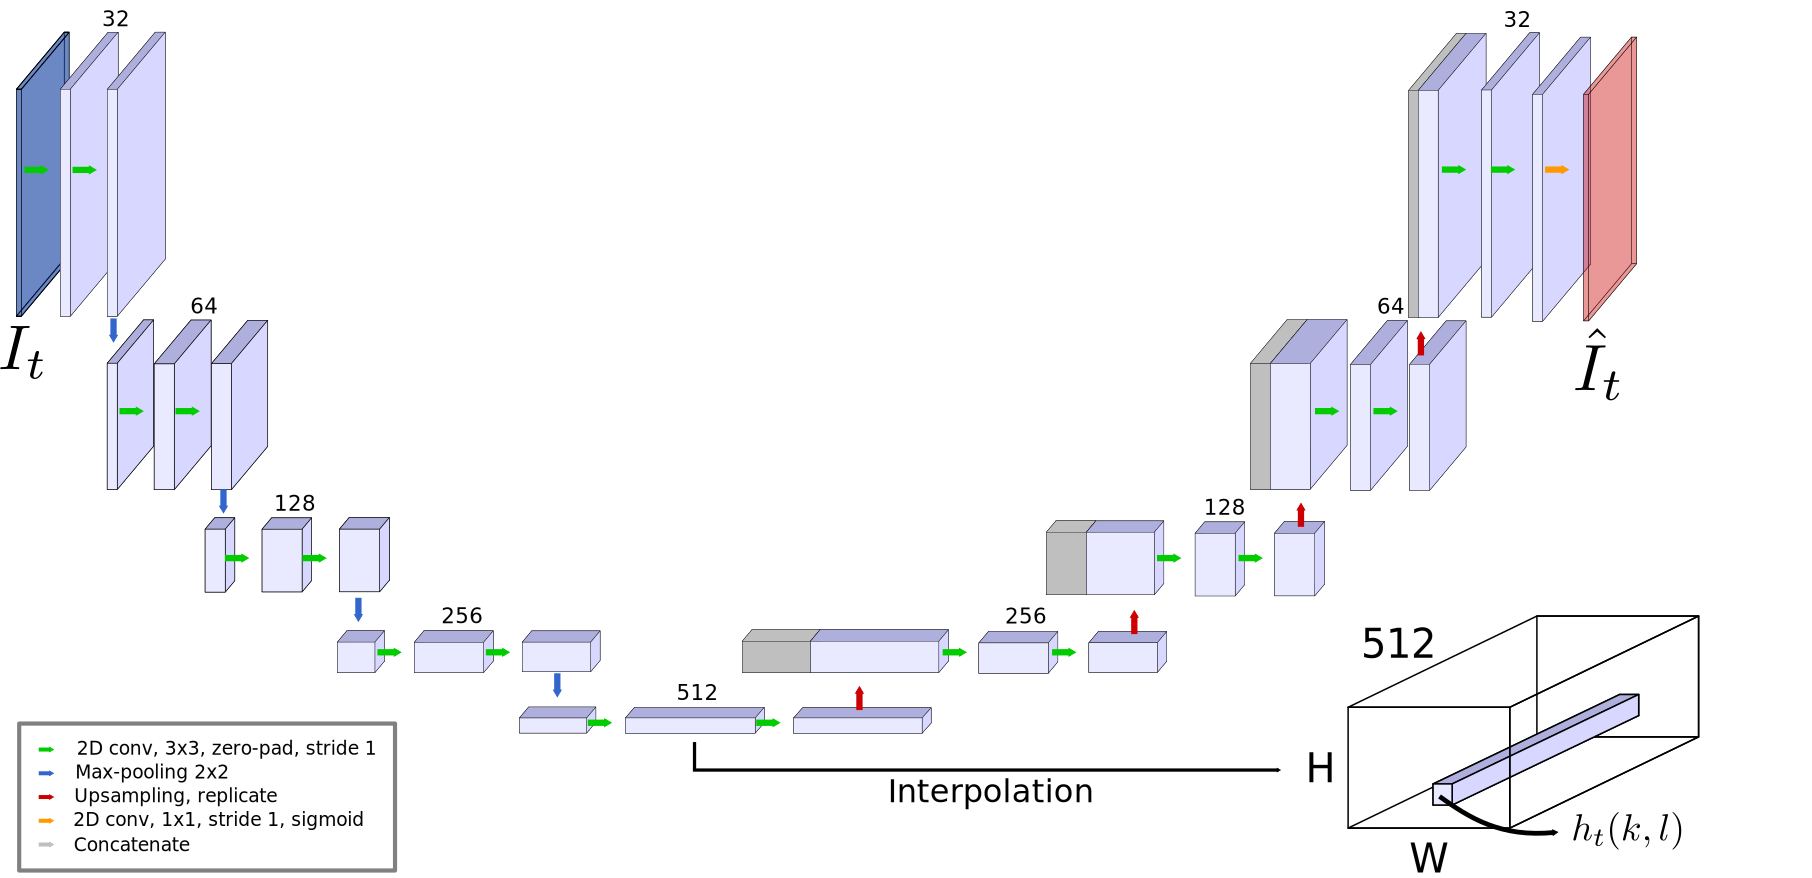
\includegraphics[width=\textwidth]{unet/model}
  \caption[Modified U-Net architecture]{U-Net architecture.
    The number of output channels is indicated above each convolutional layer.
    We add a batch normalization layer after each convolutional layer and remove the skip connections}
  \label{fig:unet_model}
\end{figure}

\subsection{Data Augmentation} \label{ch:data_gen}
We resort to data augmentation to artificially increase the training set.
In particular, we consider transformations that are likely to occur to those observed within the original sequence.
For example, considering the Slitlamp dataset, one often observes similar images that differ by rotations, shifting, and shearing.
In this case, we consider as ``reasonable'' transformations horizontal and vertical translations as well as rotations.
Conversely, as the size of the object seldom changes, scaling and zooming are not relevant transformations.
We resort to rotation, vertical/horizontal translation, and shearing.
Additionally, we added Gaussian noise for regularization.
% The parameters of these transformations are given in chapter \ref{results_data_gen}.

\clearpage
\subsection{Feature Extraction} \label{feat_extract}
Similarly to our baseline methods, we wish that our U-Net based methods construct a feature matrix $\boldsymbol{X} = [\boldsymbol{x}_1,...,\boldsymbol{x}_S]^T \in \mathbb{R}^{S \times D}$.
After training, a forward pass is performed on all image and features are taken as the output (ReLU) of the deepest layer.
Those features correspond to a downscaled version of the input image.
Hence, it must be upscaled to the original image resolution.
Each feature dimension is independently upscaled to the original image size using bicubic interpolation.
Since one pixel becomes a region, extrapolation is also needed at border regions, shown by the red circle and square in Fig. \ref{fig:feat_extract}.
As we now have a descriptor for each pixel upscaled to the same resolution as the original data, we can take the mean over all descriptors belonging to the individual superpixels with feature dimension $D=512$.
Fig. \ref{fig:feat_extract} illustrates this step.
\vspace{10pt}

\begin{figure}[htbp]
  \centering
  \includegraphics[width=\textwidth]{feat_extract/feature_extraction}
  \caption[Feature extraction model]{Illustration of feature extraction for U-Net based methods.
    The features are extracted at the output of the bottleneck.
    Those features are then upsampled on each dimension individually to obtain the input image resolution.
    The feature vector of a given superpixel is taken as the mean of all pixels that it contains.}
  \label{fig:feat_extract}
\end{figure}

\subsection{U-Net Autoencoder}
\begingroup
\setlength\intextsep{0pt}
\begin{wrapfigure}[4]{l}[0pt]{1.4cm}
\includegraphics[height=1.5cm]{icons/unet_rec.png}
\end{wrapfigure}

\textit{U-Net Autoencoder} (or \textit{U-Net AE}) considers the core model configured as an autoencoder \cite{vincent10}.
The basic idea behind autoencoders is to produce a sparse representation of the input by means of a pretext task.
In particular, it takes as input an image and must produce at the output its reconstructed version.
Let $\mathcal{I}$ be the image set and $\boldsymbol{I}_k \in [0,1]^{H \times W \times C}$ an image with height $H$, width $W$ and number of channels $C$.
Pixels are described by $\boldsymbol{I}_k(i,j,c) \in [0,1]$ with $i$ and $j$ its indices.
The reconstructed image, of same dimension as the input, is written $\boldsymbol{\hat{I}}_k$.
The network's channel dimensions is taken as $C = c_i = c_o$.
As reconstruction objective, we chose the mean-squared error (MSE).
For a minibatch of size $B$, the loss is given by:

\begin{equation}
L_{MSE} = \frac{1}{W H |\mathcal{B}|} \sum_{\boldsymbol{I}_l \in \mathcal{B}} \sum_{i,j,c} \|\boldsymbol{I}_l(i,j,c) - \boldsymbol{\hat{I}}_l(i,j,c)\|^2
\label{eq:mse_loss}
\end{equation}
\vspace{6pt}

Where $\| \cdot \|$ is the $L2$-norm and $\mathcal{B} \subset \mathcal{I}$ is the minibatch.
In later formulations, we will omit the summation on the mini-batch for clarity.

\clearpage
\subsection{U-Net Prior Autoencoder} \label{unet_gaze_rec}
\begingroup
\setlength\intextsep{0pt}
\begin{wrapfigure}[4]{l}[0pt]{1.4cm}
\includegraphics[height=1.5cm]{icons/unet_gaze_rec.png}
\end{wrapfigure}

In contrast with \textit{U-Net Autoenc}, \textit{U-Net Prior Autoencoder} (or \textit{U-Net Prior AE}) introduces a prior on the user-provided 2D location in the loss function.
Our intuition is that, in most image modalities, the object of interest covers only a small portion of the frame.
Also, the background is often homogeneous or even fully black, e.g. for CT and MRI scans.
Hence, we speculate that penalizing the loss around the 2D locations equalizes the weights given to background and object of interest in terms of the area occupied by the foreground/background, respectively.
In particular, let $\boldsymbol{g} = [g_x, g_y]$ be the xy-coordinates of a user-provided 2D location, and  $\boldsymbol{Z} \in [0,1]^{H \times W}$ a probability map.
Assuming that $\boldsymbol{g}$ is available for an image $\boldsymbol{I}$, we take $\boldsymbol{Z} \sim \mathcal{N}(\boldsymbol{g}, \sigma^2\mathbb{I})$, a 2D-Gaussian distribution with standard deviation $\sigma$ and mean $\boldsymbol{g}$.
For images where no locations are available, we use as prior a Uniform distribution:
Concretely:

\begin{equation}
\boldsymbol{Z} = 
\begin{cases}
  \mathcal{G}(\boldsymbol{g}, \sigma^2\mathbb{I}),         & \text{if $\bm{g}$ is availabe }\\
  \mathcal{U}(0,WH),& \text{otherwise}\\
\end{cases}
\label{eq:gaussian}
\end{equation}
\hspace{6pt}

The loss function is given by:

\begin{equation}
L_{MSE\_Gaze} = \frac{1}{W H} \sum_{i,j} \frac{\boldsymbol{Z}_{i,j}}{\max{\{\boldsymbol{Z}\}}} \|\boldsymbol{I}_{i,j} - \boldsymbol{\hat{I}}_{i,j}\|^2
\label{eq:mse_gaze_loss}
\end{equation}
\hspace{6pt}


\subsection{U-Net Predict Location} \label{sec:unet_pred_loc}

\begin{wrapfigure}[4]{l}[0pt]{1.4cm}
\includegraphics[height=1.5cm]{icons/unet_gaze_prob.png}
\end{wrapfigure}

\textit{U-Net Predict Location} (or \textit{U-Net Pred Loc}) is grounded on the same idea as \textit{U-Net Prior AE}, except that we rather propose to predict a probability map of the 2D location given the image.
We model the output probability map following eq. \ref{eq:gaussian}.
As loss function, we use the \gls{bce}:

\begin{equation}
L_{BCE} = -\sum_{i,j} \boldsymbol{Z}_{i,j} \log{\boldsymbol{\hat{Z}}_{i,j}}
\label{eq:ce_loss}
\end{equation}
\hspace{6pt}

\clearpage
\subsection{U-Net Predict Location Frozen}

\setlength\intextsep{0pt}
\begin{wrapfigure}[4]{l}[0pt]{1.4cm}
\includegraphics[height=1.5cm]{icons/unet_gaze_prob_freeze.png}
\end{wrapfigure}

\textit{U-Net Predict Location Frozen} (or \textit{U-Net Pred Loc Frozen}) combines the benefits of \textit{U-Net Autoenc} and \textit{U-Net Predict Location}.
The model is first trained as an autoencoder similarly to \textit{U-Net AE}.
Encoder weights are then frozen, the last layer is modified to output a single channel, and the model is re-trained in a similar fashion as \textit{U-Net Predict Location}.
This method aims at leveraging the benefits of the autoencoder setting while using the location prior as in \textit{U-Net Predict Location}.
Fig. \ref{fig:model_freeze} shows the network's portion where weights are frozen.

\begin{figure}[htbp]
  \centering
  \includegraphics[width=5.0cm]{unet/model5_coarse}
  \caption[Modified U-Net with freezed encoder part]{Illustration of frozen layers in \textit{U-Net Pred Loc Frozen} method. Frozen layers are in the highlighted in striped blue.}
  \label{fig:model_freeze}
\end{figure}

\subsection{U-Net Motion Predict} \label{sec:unet_pred_loc_concat}
\begingroup
\setlength\intextsep{0pt}
\begin{wrapfigure}[4]{l}[0pt]{1.4cm}
\includegraphics[height=1.5cm]{icons/unet_gaze_prob_concat.png}
\end{wrapfigure}

Another approach, which we call \textit{U-Net Motion Predict} (or \textit{U-Net Motion Pred}) incorporates the temporal correlation of images.
In particular, we leverage the assumption that both the object of interest and the provided 2D locations move in a smooth and coherent manner.
Concretely, let $\boldsymbol{Z}^{(t-1)}$ and $\boldsymbol{\hat{Z}}^{(t)}$ the location cues at time $t-1$ and $t$, respectively.
We assume that temporal coherence can be enforced by predicting $\boldsymbol{\hat{Z}}^{(t)}$ from $\boldsymbol{I}^{(t)}$ and $\boldsymbol{Z}^{(t-1)}$.
We implement the latter by using as input a tensor that concatenates $\boldsymbol{I}^{(t)}$ and $\boldsymbol{Z}^{(t-1)}$, so as to predict $\boldsymbol{Z}^{t}$.
Similar to \textit{U-Net Predict Location}, we use the \gls{bce} loss function.
Fig. \ref{fig:unet_gaze_concat} illustrates our method.

\begin{figure}[htbp]
  \centering
  \includegraphics[width=7cm]{unet/unet_gaze_concat}
  \caption[U-Net Motion Predict]{Structure of model \textit{U-Net Motion Predict}.
    The location probability map $\boldsymbol{Z}^{(t-1)}$ is concatenated to the current image data $\boldsymbol{I}^{(t)}$.
    The networks learns to predict the current probability map $\boldsymbol{Z}^{(t)}$.}
  \label{fig:unet_gaze_concat}
\end{figure}

\subsection{U-Net Motion Predict LSTM} \label{ch:unet_gaze_prob_lstm}
\begingroup
\setlength\intextsep{0pt}
\begin{wrapfigure}[4]{l}[0pt]{1.4cm}
\includegraphics[height=1.5cm]{icons/unet_gaze_prob_lstm}
\end{wrapfigure}

\textit{U-Net Motion Predict LSTM} (or \textit{U-Net Motion Pred LSTM}) follows the same idea as \textit{U-Net Motion Pred}, but rather considers temporal coherence over a longer period.
In particular, we instantiate $3$ models similar to \textit{U-Net Predict Location} with shared weights, and predict the three corresponding probability maps.
In parallel, we concatenate these $3$ probability maps, feed them to a recurrent unit and predict the next probability map.
As recurrent unit, we use a \gls{lstm} module \cite{shi15} with filters of size $3 \times 3$ and no return sequence.
Fig. \ref{fig:unet_gaze_lstm} illustrates our architecture.

\endgroup

\begin{figure}[htbp]
  \centering
  \includegraphics[width=10cm]{unet/unet_gaze_lstm}
  \caption[Structure of U-Net Motion Predict LSTM]{Structure of \textit{U-Net Motion Predict LSTM}.
    A sequence of three images is fed to three identical U-Net models as in \textit{U-Net Pred Location} with shared weights.
    The predicted probability maps $\boldsymbol{\hat{Z}}$ are fed to a \gls{lstm} module to predict the next probability map.}
  \label{fig:unet_gaze_lstm}
\end{figure}

The overall loss $L_{BCE\_LSTM}$ for one image sequence of three images is written:
\begin{equation}
L_{BCE\_LSTM} = \alpha \Big[\sum_{d=1}^3 L_{BCE}(\boldsymbol{\hat{Z}}^{(t-d)}, \boldsymbol{Z}^{(t-d)})\Big] + (\alpha - 1) L_{BCE}(\boldsymbol{\hat{Z}}^{(t)}, \boldsymbol{Z}^{(t)})
\label{eq:bce_lstm}
\end{equation}

Where $L_{BCE}$ is the binary cross entropy.
Parameter $\alpha$ is used to adjust the weight of the \gls{lstm} predictions.

\subsection{U-Net Based Methods Overview}
Tab. \ref{tab:summary_unet_methods} summarizes the above U-Net based methods.
% To recap, $C$ is the number of image channels ($1$ for grayscale and $3$ for colored) and $c\_i$, $c\_o$ the number of the networks input and output channels, respectively.

\begin{table}[!htbp]
   \centering
   \caption[U-Net based method overview]{Overview of U-Net based methods with $C$ the number of channels of images.}
   \begin{tabular}{l|m{1.3cm}|c|c|c|c}
      \toprule
      \textbf{Method} & \textbf{Symbol} & \textbf{Inputs} & \textbf{Outputs} & \textbf{In. chans} & \textbf{Out. chans} \\
      \midrule
      U-Net Autoencoder & \includegraphics[width=1cm]{icons/unet_rec.png} & Image & Image & $C$ & $C$ \\
      \midrule
      U-Net Prior Autoencoder & \includegraphics[width=1cm]{icons/unet_gaze_rec.png} & Image & \specialcell{Image \& \\Location-prior} & $C$ & $C$ \\
      \midrule
      U-Net Predict Location & \includegraphics[width=1cm]{icons/unet_gaze_prob.png} & Image & Location-prior & $C$ & $1$ \\
      \midrule
      U-Net Predict Location Frozen & \includegraphics[width=1cm]{icons/unet_gaze_prob_freeze.png} & Image & Location-prior & $C$ & $1$ \\
      \midrule
      U-Net Motion Predict & \includegraphics[width=1cm]{icons/unet_gaze_prob_concat.png} & \specialcell{Image \& \\Location-prior} & Location-prior & $C+1$ & $1$ \\
       \midrule
      U-Net Motion Predict LSTM & \includegraphics[width=1cm]{icons/unet_gaze_prob_lstm.png} & \specialcell{Batch of \\ Consecutive images} & Location-prior & $3 \times C$ & $3 \times 1$ \\
      \bottomrule
   \end{tabular}
   \label{tab:summary_unet_methods}
\end{table}


\section{Evaluation framework}
We now describe the evaluation framework used to compare our feature extraction methods.

\subsection{Classification setup} \label{random_forest}
We compare our methods in a \gls{pn} classification setup using a \gls{rf} binary classifier.
We evaluate using 5-fold cross-validation \cite[p. 241]{hastie09}.
Prior to every construction of fold, the samples and their corresponding labels are shuffled.
Each validation set is then evaluated using two metrics: \gls{pr} curve and F1-score.
The final performance measure is then given by the average performance over all folds.
Our pipeline is shown on Fig. \ref{fig:random_forest}.

\begin{figure}[htbp]
  \centering
  \includegraphics[width=14cm]{random_forest/random_forest}
  \caption[Evaluation pipeline]{Pipeline of the evaluation phase. We fit a \gls{rf} classifier to features $\boldsymbol{X}$, extracted on one sequence, with its corresponding ground truth labels $\boldsymbol{y}$.
    We then perform a k-fold cross-validation.}
  \label{fig:random_forest}
\end{figure}

For each tree, all nodes are expanded until the leaves are pure, as advised in \cite[pg. 596]{hastie09}
The forest has $150$ trees and pick $m=\sqrt{D}$ predictor variables, where $D$ is the feature dimension.
In the evaluation phase, each tree takes as input the evaluation samples and provides a vote.
The votes of individual trees are then averaged so as to provide a probability of being positive.

\subsection{Performance metrics}
F1-Score is a metric that computes the geometric mean between precision and recall.
It writes:

\begin{equation}
\textrm{F1-Score} = 2 \cdot \frac{\textrm{Precision} \cdot \textrm{Recall}}{\textrm{Precision} + \textrm{Recall}}
\label{eq:f1_score}
\end{equation}
\hspace{6pt}

We define the \textit{Max F1-Score}, as the maximum F1-score achieved by thresholding the output probability of our \gls{rf} over $1000$ values linearly spread within the range $[0;1]$.
An illustration is given in Fig. \ref{fig:f1_score}.

\begin{figure}[ht]
  \centering
  \includegraphics[width=11cm]{f1_score/f1_score}
  \caption[Illustration of max F1-Score]{Illustration of \textit{max F1-Score}. The left plot shows an example of a \textit{Precision Recall curve}. The diagram on the right shows the F1-Score with respect to \textit{Recall}. \textit{max F1-Score} is highlighted by a green marker.}
  \label{fig:f1_score}
\end{figure}

\subsection{Hyperparameters} \label{ch:eval_configs}
For the training of our U-Net based methods, we follow the general practice and apply random weight initialization.
As the latter step might induce variations in performance, we evaluate each method through ten training runs, i.e. each model is trained and evaluated ten times, and their performance measures are averaged.

As our baseline methods are less affected by random initialization, we compute a single feature set per method,
but train our \gls{rf} ten times on each feature set.

\subsubsection{Baseline Methods}
Tab. \ref{tab:baseline_params} shows the different parameters used for all baseline methods.
For comparison purposes, both \textit{ScSP} and \textit{BoVW}, have $512$ classes and a SIFT keypoint size of $16 \times 16$ pixels.
The number of keypoints used for vector quantization for both methods is chosen empirically.
For methods that rely on path extraction, we first define the \gls{mspw} as

\begin{equation}
   MSPW = \frac{1}{S} \sum_{i=1}^S \sqrt{A_i}
   \label{eq:mspw}
\end{equation}
\vspace{6pt}
Where $S$ is the number of superpixels in the sequence and $A_{i}$ the amount of pixels contained in superpixel $i$.
The patch size of method \textit{ScSP} is set empirically to $3 \cdot MSPW$.
For \textit{VGG-16}, we set it to $2 \cdot MSPW$.

\begin{table}[!htbp]
   \centering
   \caption[Baseline parameters]{Hyper-parameters of baseline methods}
   \begin{tabular}{c|m{1.3cm}|c|l}
      \toprule
      \textbf{Method} & \textbf{Symbol} & \textbf{\makecell{Feature \\ Dimension $D$}} & \textbf{Parameters}\\
      \midrule
      BoVW & \makecell{\includegraphics[width=1cm]{icons/bovw}} & $512$ &
        \makecell[l]{Number of classes = $512$ \\
                  SIFT KP size = $16 \times 16$px \\
                  Number of KP for CB per image = $100$} \\
      \midrule
      ScSP & \makecell{\includegraphics[width=1cm]{icons/scsp}} & $10'752$ &
        \makecell[l]{Number of classes = $512$ \\
                  SIFT KP size = $16 \times 16$px \\
                  Number of KP for CB over all sequence = $20'000$ \\
                  Pyramid levels = $[1,2,4]$ \\
                  Patch width and height = $3 \cdot MSPW$} \\
      \midrule
      VGG-16 & \makecell{\includegraphics[width=1cm]{icons/vgg}} & $4'096$ &
        \makecell[l]{Patch width and height = $2 \cdot MSPW$} \\
      \bottomrule
      \multicolumn{4}{c}{KP $\coloneqq$ keypoint \hspace{14pt} CB $\coloneqq$ codebook \hspace{14pt} MSPW $\coloneqq$ mean superpixel width} \\
      \bottomrule
   \end{tabular}
   \label{tab:baseline_params}
\end{table}
\vspace{20pt}

\subsubsection{U-Net Based Methods}
For methods that predict a probability map, we set the standard deviation $\sigma$ to $6\%$ of the image width.
For methods that use the probability map in the loss function, we set $\sigma$ to $30\%$ of the image width.
Tab. \ref{tab:unet_params} gives the values of the parameters of our U-Net based models.
\vspace{30pt}

\begin{table}[!htbp]
   \centering
   \caption[U-Net based method parameters]{Hyper-parameters of U-Net based methods.}
   \begin{tabular}{l|m{3.3cm}|l}
      \toprule
      \textbf{Method} & \textbf{\makecell{Symbol}} & \textbf{Parameters}\\
      \midrule
      U-Net AE Prior & \makecell{\includegraphics[width=1cm]{icons/unet_gaze_rec}} &
        \makecell[l]{$\sigma = 30\%$ of image width} \\
      \midrule
        \makecell[l]{U-Net AE Prior \\
                     U-Net Pred Loc Freeze \\
                     U-Net Motion Pred} &
      \makecell{\includegraphics[width=1cm]{icons/unet_gaze_prob} \includegraphics[width=1cm]{icons/unet_gaze_prob_freeze} \includegraphics[width=1cm]{icons/unet_gaze_prob_concat}} &
        \makecell[l]{$\sigma = 6\%$ of image width} \\
      \midrule
      U-Net Motion Pred LSTM & \makecell{\includegraphics[width=1cm]{icons/unet_gaze_prob_lstm}} &
        \makecell[l]{$\sigma = 6\%$ of image width \\
                     $\alpha = 0.2$} \\
      \bottomrule
   \end{tabular}
   \label{tab:unet_params}
\end{table}

All of our U-Net based models are trained for $20$ epochs using the Adam optimizer \cite{kingma15}.
We set the learning rate to $0.0001$.
Weights are initialized with the Glorot method \cite{glorot10}.
The batch size is set according to the model architecture and the input size.
\vspace{30pt}

\clearpage
\subsubsection{Data Augmentation} \label{results_data_gen}

The data augmentation parameters are given in Tab. \ref{tab:data_gen_param}.
Example frames are shown in \ref{fig:data_gen}.

\begin{table}[!htbp]
   \centering
   \caption[Data augmentation parameters]{Parameters of data augmentation. Rotation, translation, shearing, and gaussian noise are used as transformation.}
   \begin{tabular}{l|c}
      \toprule
      \textbf{Parameter} & \textbf{Value} \\
      \midrule
      Rotation range & $\pm11.25$° \\
      \midrule
      Horizontal translation range & $20\%$ of image width \\
      \midrule
      Vertical translation range & $20\%$ of image height \\
      \midrule
      Shearing range & $\pm22.5$° \\
      \midrule
     Gaussian noise & $0.5\%$ of average variance on each channel\\
      % \midrule
      % Number of samples per epoch & $2'000$ \\
      \bottomrule
   \end{tabular}
   \label{tab:data_gen_param}
\end{table}
\vspace{30pt}

\begin{figure}[!htbp]
  \centering
  \includegraphics[width=\textwidth]{unet/data_gen}
  \caption[Examples of data generator]{Examples of data augmentation on \textit{Slitlamp}. We used rotation, translation, shearing and added Gaussian noise.}
  \label{fig:data_gen}
\end{figure}

%%% Local Variables:
%%% mode: latex
%%% TeX-master: "../../main"
%%% End:
